%%%%%%%%%%%%%%%%%%%%%%%%%%%%%%%%%%%%%%%%%%%%%%%%%%%%%%%%%%%%%%%%%%%%%%%%%%%
%% This file is part of the book
%%
%% Algorithmic Graph Theory
%% http://code.google.com/p/graph-theory-algorithms-book/
%%
%% Copyright (C) 2009, 2010, 2011 Minh Van Nguyen <nguyenminh2@gmail.com>
%%
%% See the file COPYING for copying conditions.
%%%%%%%%%%%%%%%%%%%%%%%%%%%%%%%%%%%%%%%%%%%%%%%%%%%%%%%%%%%%%%%%%%%%%%%%%%%

\documentclass{article}

\usepackage{tikz}
\usetikzlibrary{external}
\tikzexternalize{social-network}

\begin{document}

\begin{figure}
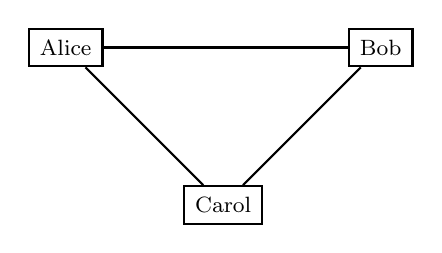
\begin{tikzpicture}
[lineDecorate/.style={-,thick},%
  nodeDecorate/.style={shape=rectangle,inner sep=4pt,draw,thick}]
%% nodes or vertices
\foreach \nodename/\x/\y in {Alice/-2/2, Bob/2/2, Carol/0/0}
{
  \node (\nodename) at (\x,\y) [nodeDecorate] {\footnotesize\nodename};
}
%% edges or lines
\path
\foreach \startnode/\endnode in {Alice/Bob, Alice/Carol, Bob/Carol}
{
  (\startnode) edge[lineDecorate] node {} (\endnode)
};
\end{tikzpicture}
\end{figure}

\end{document}
